\newpage
\section{Test 3}
\label{Sec:test_3}

In the third test setting rover's parcour is divided into six time intervals with different values of torques applied to the wheels:

\begin{enumerate} 
  \item $0s < t_s < 50s$, $\tau = 0N$           
  \item $50s < t_s < 100s$, $\tau = 700N$        
  \item $100s < t_s < 150s$, $\tau = 0N$         
  \item $150s < t_s < 220s$, $\tau = -500N$
  \item $220s < t_s < 300s$, $\tau = 0N$         
  \item $300s < t_s < 400s$, $\tau = -500N$ 
\end{enumerate}

\noindent Other external forces acting on the rover are the gravity and ground reaction. Initial position of the center of mass of the robot
has been set to (x, y, z) = (18, 0.55, 10). In the $5^{th}$ phase rover effectively stops its motion until negative torques are applied.

\begin{figure}[H]
  \centering
    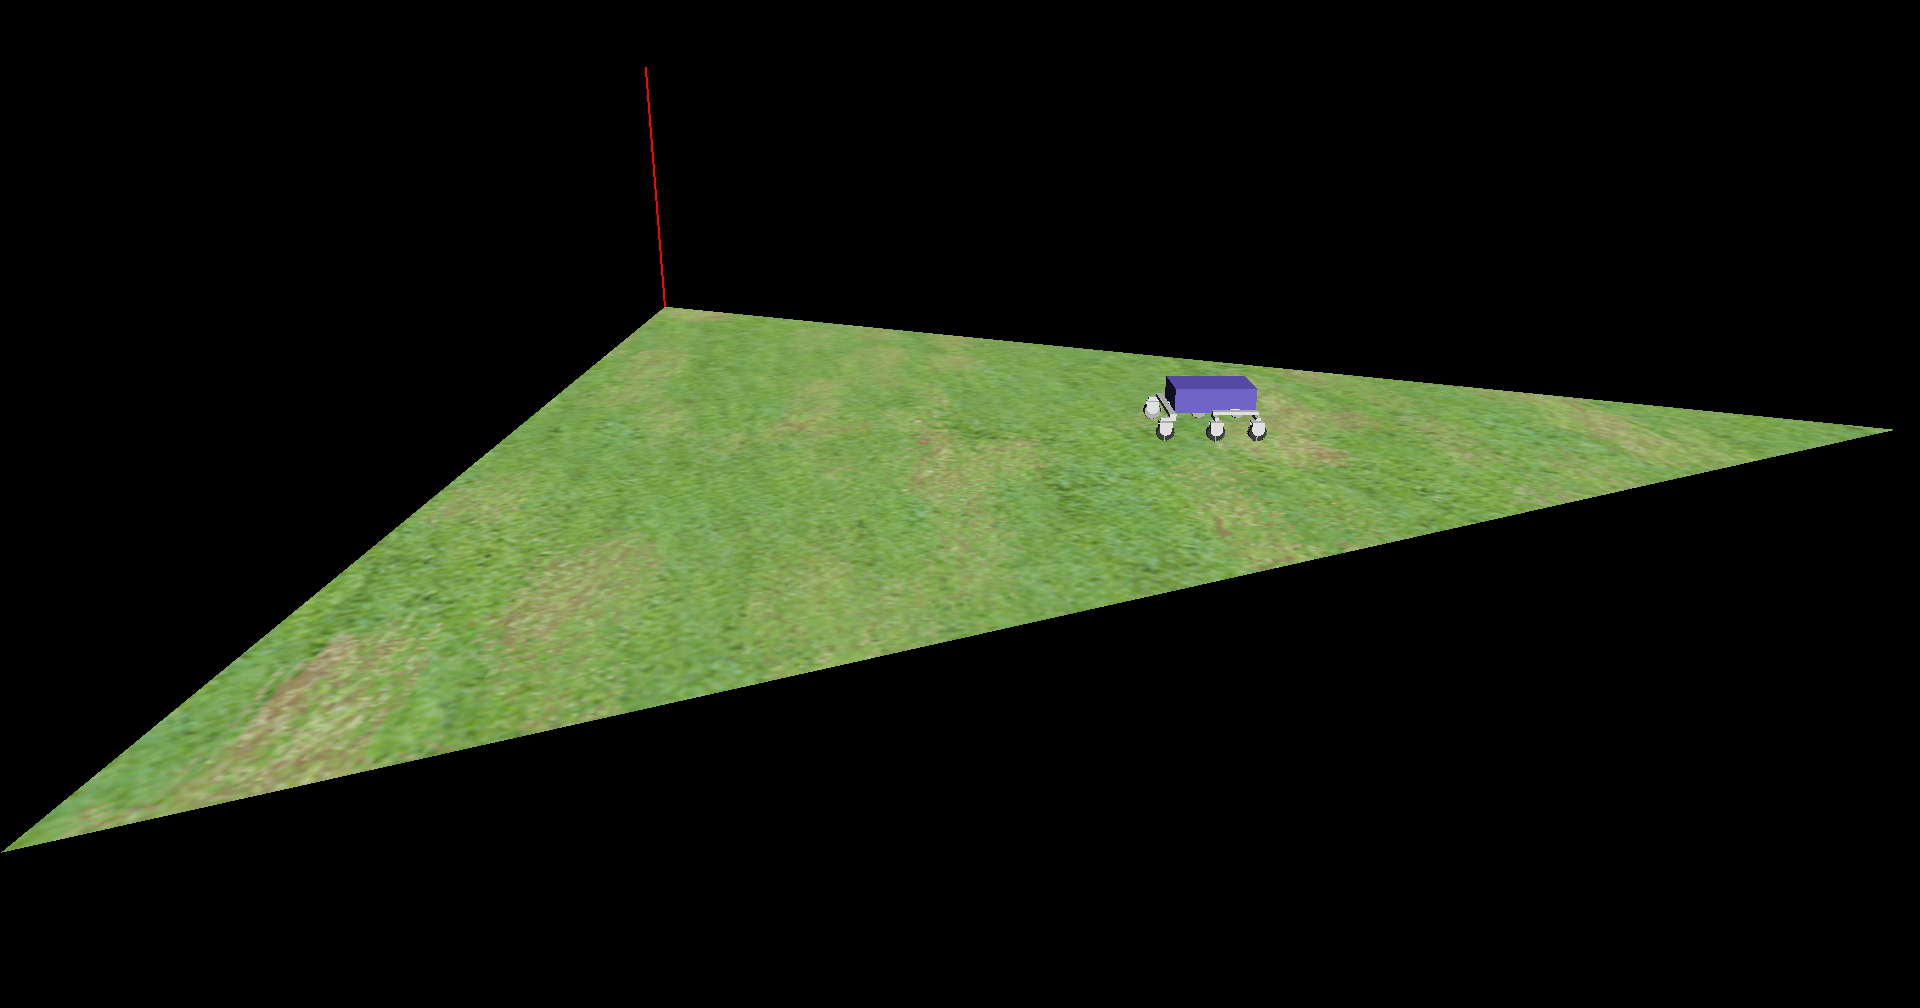
\includegraphics[width=0.8\textwidth]{run_1}
  \caption{Third test scenario}
\end{figure}

\noindent In this case, following quantities have been plotted:

\begin{itemize}
  \item $x_{COM}$ - mass center coordinates
\end{itemize}

\begin{figure}[H]
  \centering
    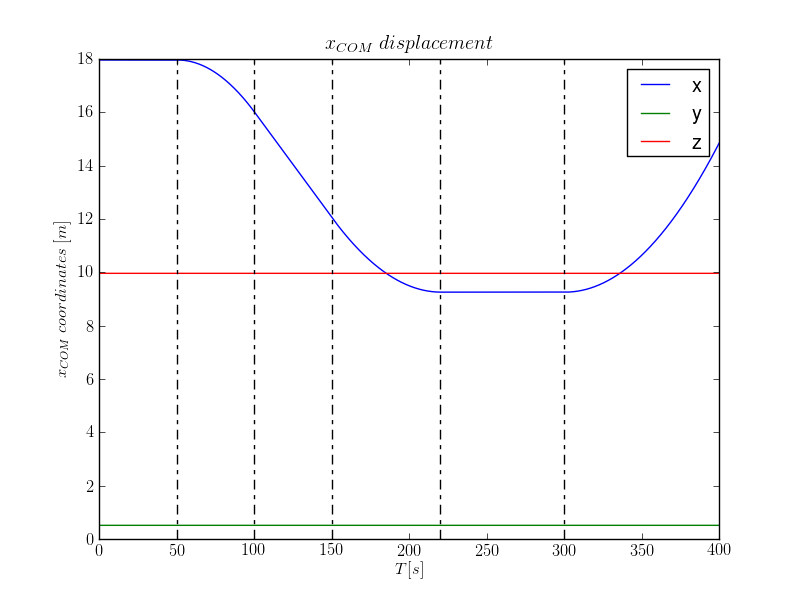
\includegraphics[width=0.8\textwidth]{xCOM3}
  \caption{$x_{COM}$}
\end{figure}

\begin{itemize}
  \item $x_{wheels}$ - wheels angular displacement 
\end{itemize}

\begin{figure}[H]
  \centering
    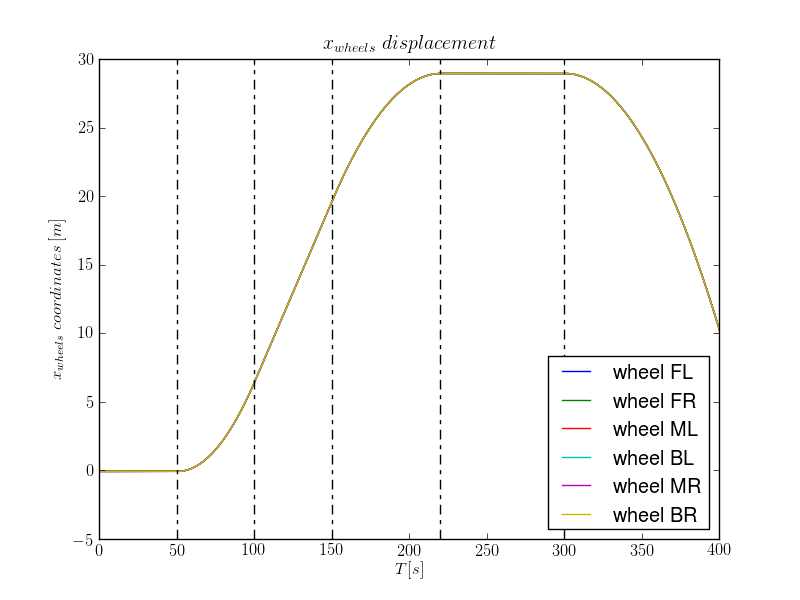
\includegraphics[width=0.8\textwidth]{xWHEELS3}
  \caption{$x_{wheels}$}
\end{figure}

\begin{itemize}
  \item $v_{COM}$ - mass center velocity
\end{itemize}

\begin{figure}[H]
  \centering
    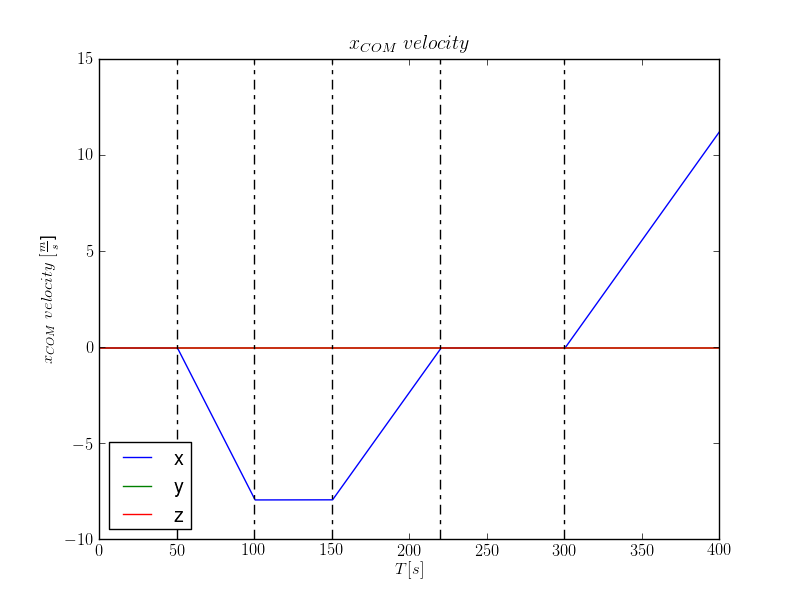
\includegraphics[width=0.8\textwidth]{vCOM3}
  \caption{$v_{COM}$}
\end{figure}

\begin{itemize}
  \item $v_{wheels}$ - wheels angular velocity
\end{itemize}

\begin{figure}[H]
  \centering
    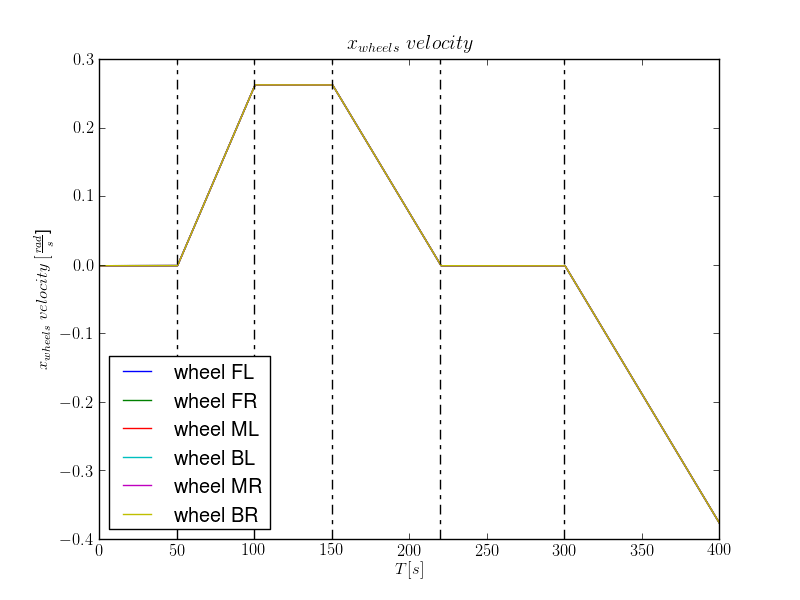
\includegraphics[width=0.8\textwidth]{vWHEELS3}
  \caption{$v_{wheels}$}
\end{figure}

\begin{itemize}
  \item $R_{COM}$ - reaction forces of center of mass in lagrangian coordinates
\end{itemize}

\begin{figure}[H]
  \centering
    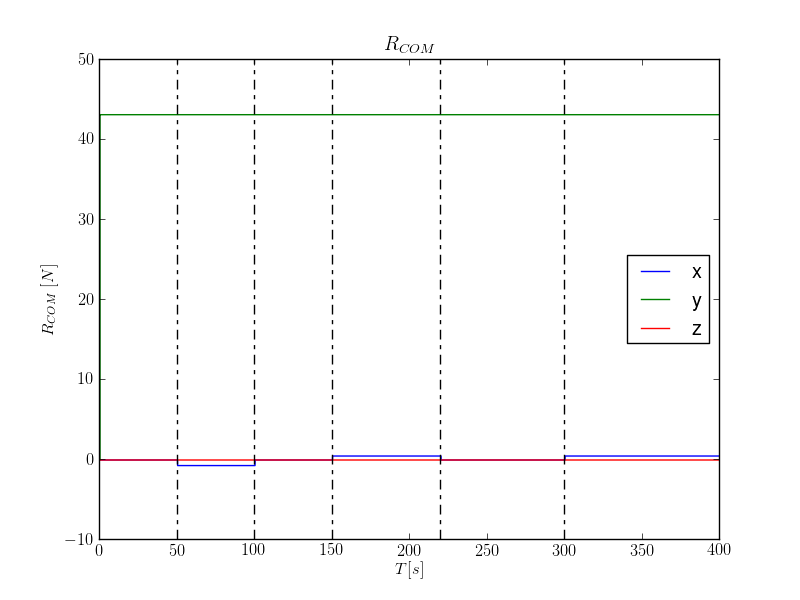
\includegraphics[width=0.8\textwidth]{pCOM3}
  \caption{$R_{COM}$}
\end{figure}

\begin{itemize}
  \item $R_{wheels}$ - reaction forces of wheels in lagrangian coordinates
\end{itemize}

\begin{figure}[H]
  \centering
    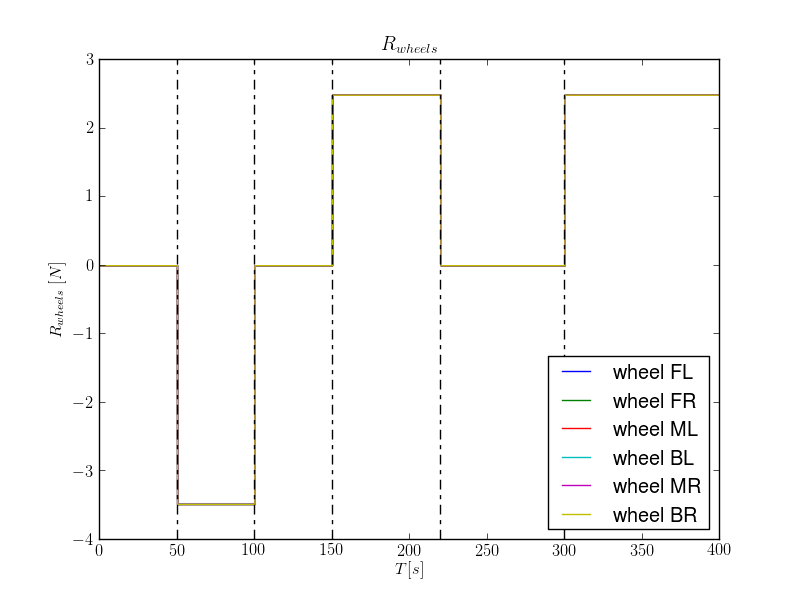
\includegraphics[width=0.8\textwidth]{pWHEELS3}
  \caption{$R_{wheels}$}
\end{figure}

\begin{itemize}
  \item $\lambda_{N}$ - normal component of the contact force (impulsion) for each wheel
\end{itemize}

\begin{figure}[H]
  \centering
    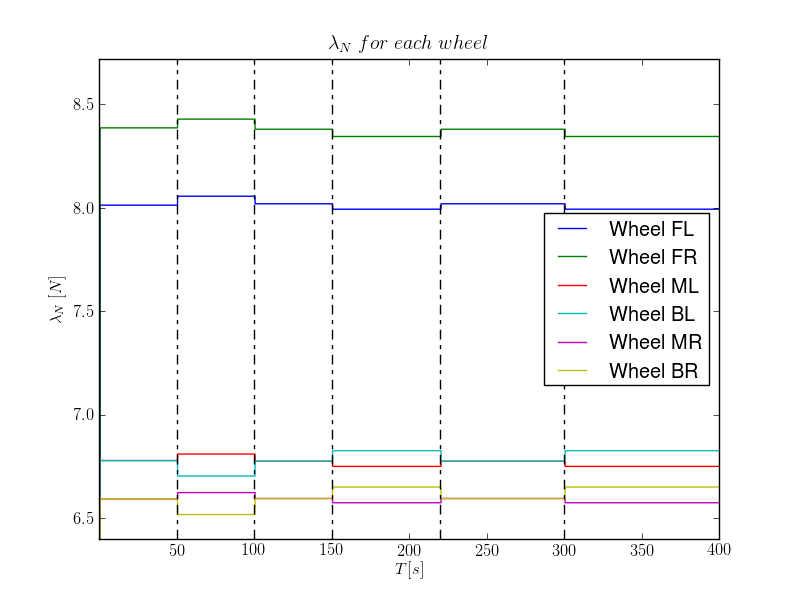
\includegraphics[width=0.8\textwidth]{lambdaN3}
  \caption{$\lambda_N$}
\end{figure}

\begin{itemize}
  \item $\lambda_{T_x}$ - tangential component of the contact force in the x direction for each wheel
\end{itemize}

\begin{figure}[H]
  \centering
    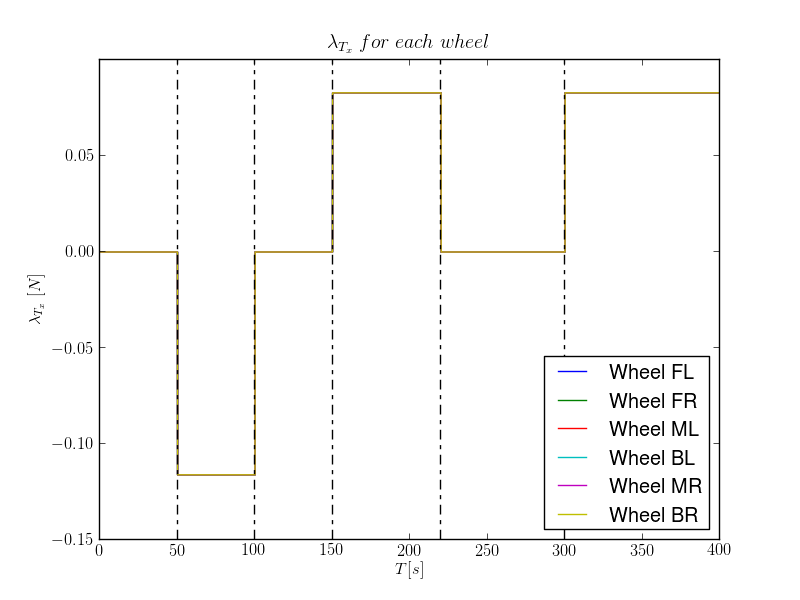
\includegraphics[width=0.8\textwidth]{lambdaTx3}
  \caption{$\lambda_{T_x}$}
\end{figure}

\begin{itemize}
  \item $\lambda_{T_z}$ - tangential component of the contact force in the z direction for each wheel
\end{itemize}

\begin{figure}[H]
  \centering
    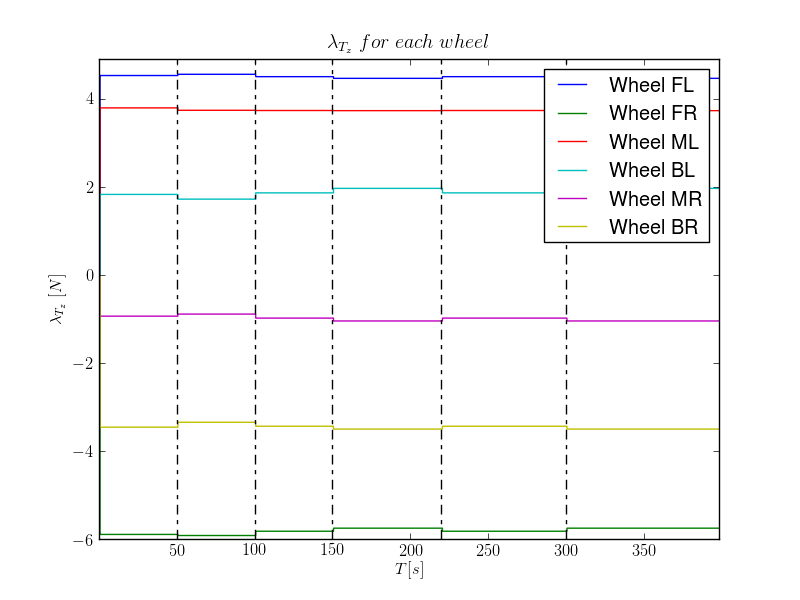
\includegraphics[width=0.8\textwidth]{lambdaTz3}
  \caption{$\lambda_{T_z}$}
\end{figure}

\begin{itemize}
  \item $y_{N}$ - gap function (distance between contact point and the constraint function) for each wheel
\end{itemize}

\begin{figure}[H]
  \centering
    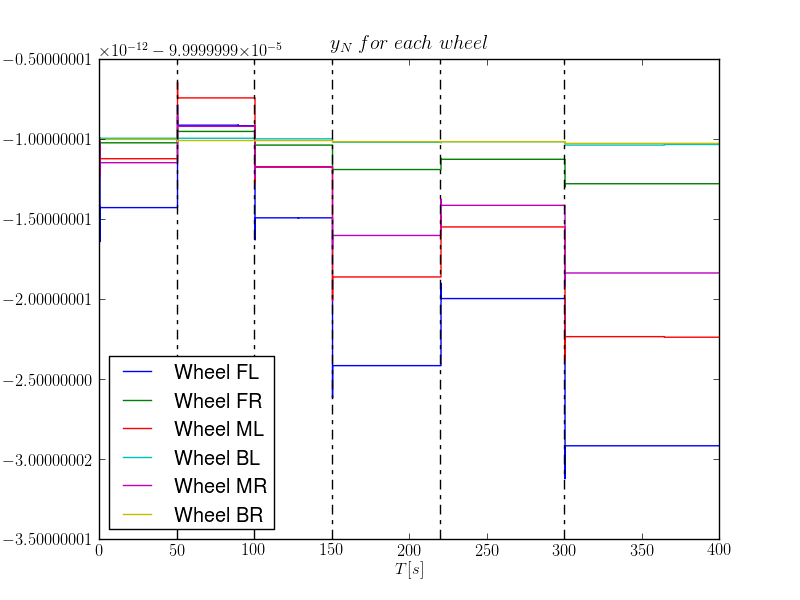
\includegraphics[width=0.8\textwidth]{yN3}
  \caption{$y_N$}
\end{figure}

\begin{itemize}
  \item $\dot{y}_{N}$ - normal component of the local contact velocity for each wheel
\end{itemize}

\begin{figure}[H]
  \centering
    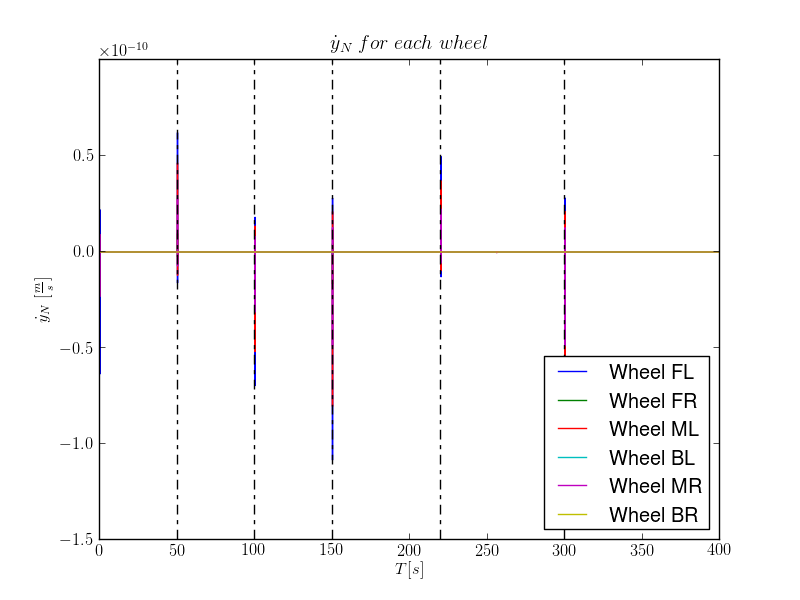
\includegraphics[width=0.8\textwidth]{yNdot3}
  \caption{$\dot{y}_{N}$}
\end{figure}

\begin{itemize}
  \item $\dot{y}_{T_x}$ - tangential component x of the local contact velocity for each wheel
\end{itemize}

\begin{figure}[H]
  \centering
    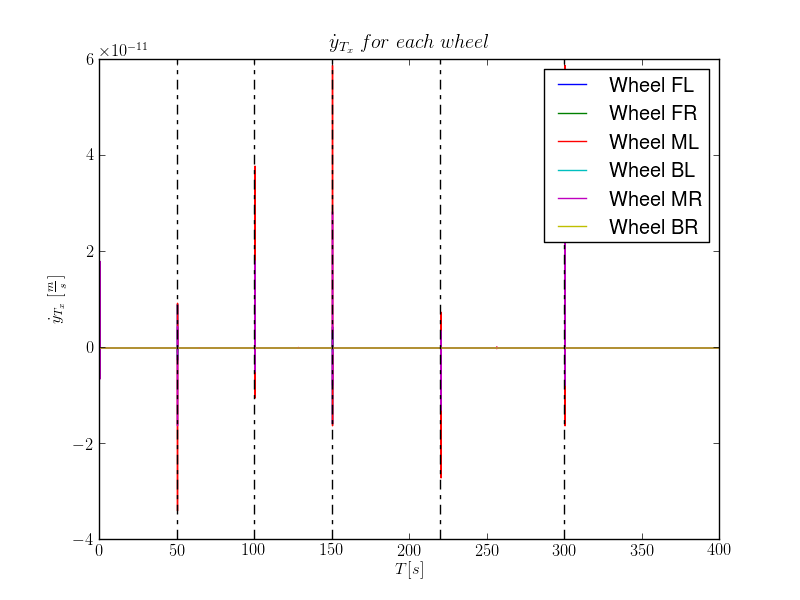
\includegraphics[width=0.8\textwidth]{yTxdots3}
  \caption{$\dot{y}_{T_x}$}
\end{figure}

\begin{itemize}
  \item $\dot{y}_{T_z}$ - tangential component z of the local contact velocity for each wheel
\end{itemize}

\begin{figure}[H]
  \centering
    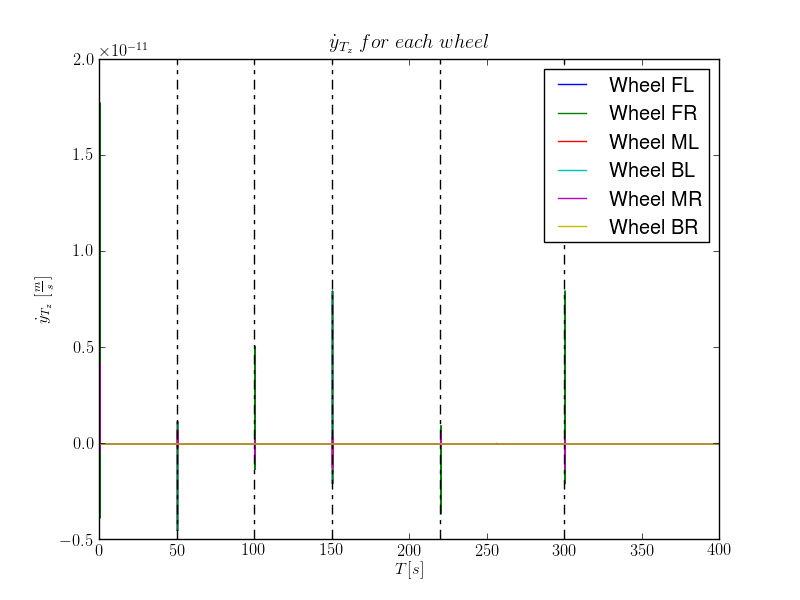
\includegraphics[width=0.8\textwidth]{yTzdots3}
  \caption{$\dot{y}_{T_z}$}
\end{figure}
